\chapter{几何着色器(The Geometry Shader)}
\begin{flushleft}
假设我们没有使用曲面细分阶段,几何着色器阶段是位于顶点和像素着色器阶段之间的可选阶段。顶点着色器输入顶点时,几何着色器输入整个基本体(primitives)。 例如,如果我们绘制三角形列表,那么概念上将为列表中的每个三角形$T$执行几何着色器程序:\\
\end{flushleft}

\begin{lstlisting}
for (UINT i = 0; i < numTriangles; ++i)
  OutputPrimitiveList = GeometryShader(T[i].vertexList);
\end{lstlisting}

\begin{flushleft}
请注意,每个三角形的三个顶点都输入到几何着色器中,几何着色器输出一个基元列表(list of primitives)。 与不能破坏或创建顶点的顶点着色器不同,几何着色器的主要优点是它可以创建或破坏几何体; 这样就可以在GPU上实现一些有趣的效果。 例如,输入基元(primitive)可以扩展为一个或多个其他基元,或者几何着色器可以选择不基于某些条件输出基元。 注意,输出基元不需要与输入基元的类型相同; 例如,几何着色器的常见应用是将点扩展为四边形(两个三角形)。\\

从几何着色器输出的基元由顶点列表定义。 离开几何着色器的顶点位置必须转换为齐次剪辑空间。 在几何着色器阶段之后,我们有一个顶点列表,用于定义齐次剪辑空间中的基元。 投影这些顶点(齐次分割 homogeneous devide),然后像往常一样发生光栅化。
\end{flushleft}

{\large Objectives:}
\begin{itemize}
    \item 1.了解如何编程几何着色器。
    \item 2.了解如何使用几何着色器有效地实现广告牌。
    \item 3.识别自动生成的基元ID及其某些应用程序。
    \item 4.了解如何创建和使用纹理数组,并了解它们的用途。
    \item 5.要了解alpha-to-coverage如何帮助解决alpha截断的锯齿问题。
\end{itemize}

%-------- 12.1 --------
\section{几何着色器编程(Programming Geometry Shaders)}
\begin{flushleft}
几何着色器编程很像顶点或像素着色器编程,但存在一些差异。以下代码显示了一般形式:\\
\end{flushleft}

\begin{lstlisting}
[maxvertexcount(N)]
void ShaderName (
    PrimitiveType InputVertexType InputName [NumElements],
    inout StreamOutputObject<OutputVertexType> OutputName)
{
    // Geometry shader body...
}
\end{lstlisting}

\begin{flushleft}
我们必须首先指定几何着色器将为单个调用输出的最大顶点数(每个基元调用几何着色器)。 这是通过使用以下属性语法在着色器定义之前设置最大顶点计数来完成的:\\
\end{flushleft}

\begin{lstlisting}
[maxvertexcount(N)]
\end{lstlisting}

\begin{flushleft}
其中$N$是几何着色器为单次调用输出的最大顶点数。几何着色器每次调用可以输出的顶点数是可变的,但不能超过定义的最大值。出于性能考虑,maxvertexcount 应尽可能小; [NVIDIA08]指出GS的峰值性能出现在GS输出1-20标量之间,如果GS输出在27-40个标量之间,性能会下降到50%。每次调用的标量输出数量是maxvertexcount和输出顶点类型结构中标量数量的乘积。在实践中使用这些限制很困难,因此我们可以接受低于峰值的性能,或者选择不使用几何着色器的替代实现;但是,我们还必须考虑替代实现可能具有其他缺点,这仍然可以使几何着色器实现成为更好的选择。此外,[NVIDIA08]中的建议来自2008年(第一代几何着色器),因此现在应该有所改进。\\

几何着色器采用两个参数:输入参数和输出参数。 (实际上,它可能需要更多,这是单独讨论的主题,参见§12.2.4。)输入参数始终是一个顶点数组,它定义一个基元——一个顶点,一个线为两个顶点,三个为a 三角形,四个用于邻接的线,六个用于相邻的三角形。 输入顶点的顶点类型是顶点着色器返回的顶点类型(例如,VertexOut)。 输入参数必须以基本类型为前缀,描述输入到几何着色器中的基元类型。 这可以是以下任何一种:\\
\end{flushleft}

\begin{itemize}
  \item 1.point: 输入基元是点。
  \item 2.line: 输入基元是线段(列表或条带)。
  \item 3.triangle: 输入基元是三角形(列表或条带)。
  \item 4.lineadj: 输入基元是邻接线段(列表或条带)。
  \item 5.triangleadj: 输入基元是邻接三角(列表或条带)。
\end{itemize}

\begin{flushleft}
~\\
NOTICE: 几何着色器中的输入基元始终是完整基元(例如,线的两个顶点和三角形的三个顶点)。 因此,几何着色器不需要区分列表和条带。 例如,如果要绘制三角形条带,则仍会对条带中的每个三角形执行几何着色器,并且每个三角形的三个顶点将作为输入传递到几何着色器中。 这需要额外的开销,因为多个基元共享的顶点在几何着色器中被多次处理。
~\\
输出参数始终具有inout修饰符。 此外,输出参数始终是流类型(stream type)。 流类型存储顶点列表,这些顶点定义几何着色器输出的几何。 几何着色器使用内在的Append方法将一个顶点添加到传出流列表:\\
\end{flushleft}

\begin{lstlisting}
void StreamOutputObject<OutputVertexType>::Append(OutputVertexType v);
\end{lstlisting}

\begin{flushleft}
流类型是模板类型,其中template参数用于指定传出顶点的顶点类型(例如,GeoOut)。 有三种可能的流类型:\\
\end{flushleft}

\begin{itemize}
  \item 1.PointStream<OutputVertexType>: 一个顶点列表定义的点列表(point list)
  \item 2.LineStream<OutputVertexType>: 一个顶点列表定义的线段条带(line strip)
  \item 3.TriangleStream<OutputVertexType>: 一个顶点列表定义的三角条带(triangle strip)
\end{itemize}

\begin{flushleft}
由几何着色器输出的顶点形成基元; 输出基元的类型由流类型(PointStream,LineStream,TriangleStream)指定。 对于线和三角形,输出基元始终是条带。 但是,可以使用内部RestartStrip方法模拟线和三角形列表:\\
\end{flushleft}

\begin{lstlisting}
void StreamOutputObject<OutputVertexType>::RestartStrip();
\end{lstlisting}

\begin{flushleft}
例:如果你想输出三角列表,那么你每次将三个顶点追加到输出流之后都需要调用 RestartStrip 方法。\\

下面是几何着色器签名的例子:\\
\end{flushleft}

\begin{lstlisting}
// EXAMPLE 1: GS ouputs at most 4 vertices. The input
// primitive is a line.
// The output is a triangle strip.
//
[maxvertexcount(4)]
void GS(line VertexOut gin[2],
    inout TriangleStream<GeoOut> triStream)
{
    // Geometry shader body…
}
//
// EXAMPLE 2: GS outputs at most 32 vertices. The
// input primitive is a triangle. The output 
// is a triangle strip.
//
[maxvertexcount(32)]
void GS(triangle VertexOut gin[3],
    inout TriangleStream<GeoOut> triStream)
{
    // Geometry shader body…
}
//
// EXAMPLE 3: GS outputs at most 4 vertices. The input
// primitive is a point. The output is a triangle strip.
//
[maxvertexcount(4)]
void GS(point VertexOut gin[1],
    inout TriangleStream<GeoOut> triStream)
{
    // Geometry shader body…
}
\end{lstlisting}

\begin{figure}[h]
    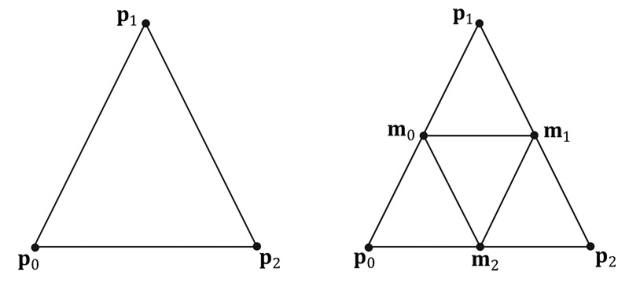
\includegraphics[width=\textwidth]{12-1}
    \centering
    \caption{将三角形细分为四个大小相等的三角形。 观察到三个新顶点是沿着原始三角形边缘的中点。}
    \label{fig:12-1}
\end{figure}

\begin{flushleft}
以下几何着色器说明了Append和RestartStrip方法; 它输入一个三角形,将其细分(图\ref{fig:12-1})并输出四个细分的三角形:\\
\end{flushleft}

\begin{lstlisting}
struct VertexOut
{
    float3 PosL : POSITION;
    float3 NormalL : NORMAL;
    float2 Tex : TEXCOORD;
};
struct GeoOut
{
    float4 PosH : SV_POSITION;
    float3 PosW : POSITION;
    float3 NormalW : NORMAL;
    float2 Tex : TEXCOORD;
    float FogLerp : FOG;
};
void Subdivide(
    VertexOut inVerts[3], 
    out VertexOut
    outVerts[6])
{
    //       1
    //       *
    //     /   \
    //    /     \
    //   m0*–—--*m1
    //  /   \   / \
    // /     \ /   \
    // *–—*–—*
    // 0     m2     2
    VertexOut m[3];
    // Compute edge midpoints.
    m[0].PosL = 0.5f*(inVerts[0].PosL+inVerts[1].PosL);
    m[1].PosL = 0.5f*(inVerts[1].PosL+inVerts[2].PosL);
    m[2].PosL = 0.5f*(inVerts[2].PosL+inVerts[0].PosL);
    // Project onto unit sphere
    m[0].PosL = normalize(m[0].PosL);
    m[1].PosL = normalize(m[1].PosL);
    m[2].PosL = normalize(m[2].PosL);
    // Derive normals.
    m[0].NormalL = m[0].PosL;
    m[1].NormalL = m[1].PosL;
    m[2].NormalL = m[2].PosL;
     // Interpolate texture coordinates.
    m[0].Tex = 0.5f*(inVerts[0].Tex+inVerts[1].Tex);
    m[1].Tex = 0.5f*(inVerts[1].Tex+inVerts[2].Tex);
    m[2].Tex = 0.5f*(inVerts[2].Tex+inVerts[0].Tex);
    outVerts[0] = inVerts[0];
    outVerts[1] = m[0];
    outVerts[2] = m[2];
    outVerts[3] = m[1];
    outVerts[4] = inVerts[2];
    outVerts[5] = inVerts[1];
};
void OutputSubdivision(VertexOut v[6],
    inout TriangleStream<GeoOut> triStream)
{
    GeoOut gout[6];
    [unroll]
    for(int i = 0; i < 6; ++i)
    {
        // Transform to world space space.
        gout[i].PosW = mul(float4(v[i].PosL, 1.0f),
        gWorld).xyz;
        gout[i].NormalW = mul(v[i].NormalL, (float3x3)gWorldInvTranspose);
        // Transform to homogeneous clip space.
        gout[i].PosH = mul(float4(v[i].PosL, 1.0f),
        gWorldViewProj);
        gout[i].Tex = v[i].Tex;
    }
    //       1
    //       *
    //     /   \
    //    /     \
    //   m0*–—--*m1
    //  /   \   / \
    // /     \ /   \
    // *–—*–—*
    // 0     m2     2
    // We can draw the subdivision in two strips:
    // Strip 1: bottom three triangles
    // Strip 2: top triangle
    [unroll]
    for(int j = 0; j < 5; ++j)
    {
        triStream.Append(gout[j]);
    }
    triStream.RestartStrip();
    triStream.Append(gout[1]);
    triStream.Append(gout[5]);
    triStream.Append(gout[3]);
}
[maxvertexcount(8)]
void GS(triangle VertexOut gin[3], inout
    TriangleStream<GeoOut>)
{
    VertexOut v[6];
    Subdivide(gin, v);
    OutputSubdivision(v, triStream);
}
\end{lstlisting}

\begin{flushleft}
几何着色器的编译方式与顶点和像素着色器非常相似。 假设我们在TreeSprite.hlsl中有一个名为GS的几何着色器,那么我们将着色器编译为字节码,如下所示:\\
\end{flushleft}

\begin{lstlisting}
mShaders["treeSpriteGS"] = d3dUtil::CompileShader(
    L"Shaders\\TreeSprite.hlsl", nullptr, "GS", "gs_5_0");
\end{lstlisting}

\begin{flushleft}
与顶点和像素着色器一样,给定的几何着色器作为管道状态对象(PSO)的一部分绑定到渲染管道:\\
\end{flushleft}

\begin{lstlisting}
D3D12_GRAPHICS_PIPELINE_STATE_DESC treeSpritePsoDesc =
    opaquePsoDesc;
...
treeSpritePsoDesc.GS =
{
    reinterpret_cast<BYTE*>(mShaders["treeSpriteGS"]->
        GetBufferPointer()),
    mShaders["treeSpriteGS"]->GetBufferSize()
};
\end{lstlisting}

\begin{flushleft}
~\\
NOTICE: 给定输入基元,几何着色器可以选择不根据某些条件输出它。 通过这种方式,几何体被几何着色器"破坏",这对某些算法很有用。\\
~\\

NOTICE: 如果没有输出足够的顶点来完成几何着色器中的基元,则会丢弃部分基元。\\
\end{flushleft}

%-------- 12.2 --------
\section{树广告牌演示(Tree Billboards demo)}
%-------- 12.2.1 --------
\subsection{概览(Overview)}
\begin{flushleft}
当树木很远时,使用广告牌技术来提高效率。 也就是说,不是渲染完全3D树的几何图形,而是在其上绘制带有3D树图片的四边形(参见图\ref{fig:12-2})。 从远处看,您无法分辨出正在使用的广告牌。 然而,诀窍是确保广告牌始终面向相机(否则达不到欺骗人眼的目的)。
\end{flushleft}

\begin{figure}[h]
    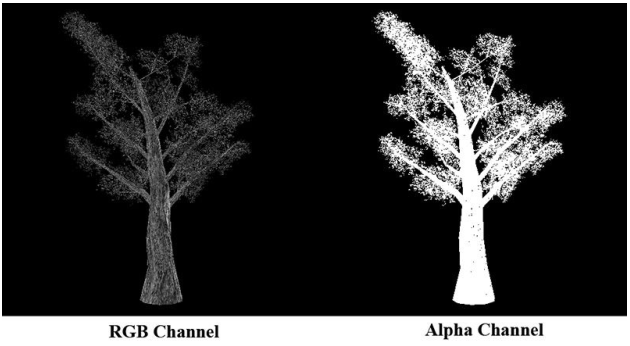
\includegraphics[width=\textwidth]{12-2}
    \centering
    \caption{一个alpha通道的树广告牌纹理}
    \label{fig:12-2}
\end{figure}

\begin{flushleft}
假设$y$轴向上并且$xz$平面是地平面,则树广告牌通常将与$y$轴对齐并且恰好面向$xz$平面中的相机。 图\ref{fig:12-3}显示了鸟瞰图中几个广告牌的局部坐标系,请注意广告牌正在"看"相机。\\
\end{flushleft}

\begin{figure}[h]
    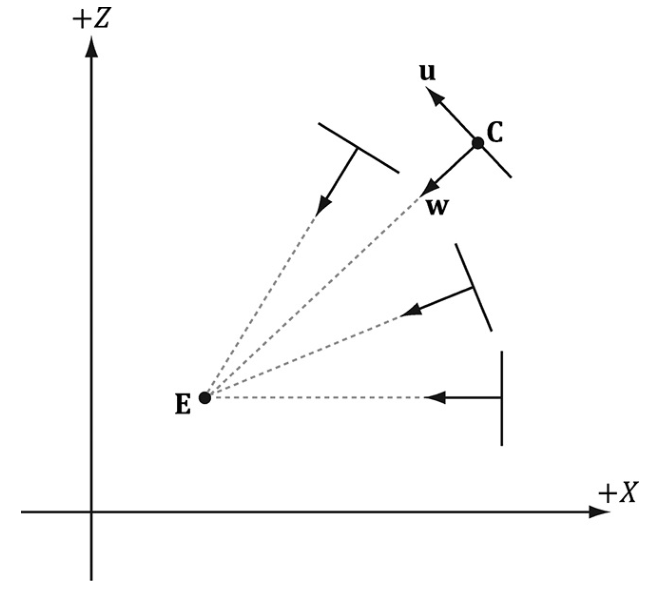
\includegraphics[width=\textwidth]{12-3}
    \centering
    \caption{树广告牌朝向相机}
    \label{fig:12-3}
\end{figure}

\begin{flushleft}
因此,假设世界空间中广告牌的中心位置$C=(C_{x},C_{y},C_{z})$和世界空间中相机$E=(E_{x},E_{y},E_{z})$的位置,我们有足够的信息描述广告牌相对于世界空间的局部坐标系:\\
\end{flushleft}

\begin{align*}
W&=\frac{(E_{x}-C_{x},0,E_{z}-C_{z})}{||(E_{x}-C_{x},0,E_{z}-C_{z})||}\\
v&=(0,1,0)\\
u&=v\times w
\end{align*}

\begin{flushleft}
给定广告牌相对于世界空间的局部坐标系,以及广告牌的世界尺寸,广告牌四边形顶点可以如下获得(见图\ref{fig:12-4}):\\
\end{flushleft}

\begin{lstlisting}
v[0] = float4(gin[0].CenterW + halfWidth*right - halfHeight*up, 1.0f);
v[1] = float4(gin[0].CenterW + halfWidth*right + halfHeight*up, 1.0f);
v[2] = float4(gin[0].CenterW - halfWidth*right - halfHeight*up, 1.0f);
v[3] = float4(gin[0].CenterW - halfWidth*right + halfHeight*up, 1.0f);
\end{lstlisting}

\begin{figure}[h]
    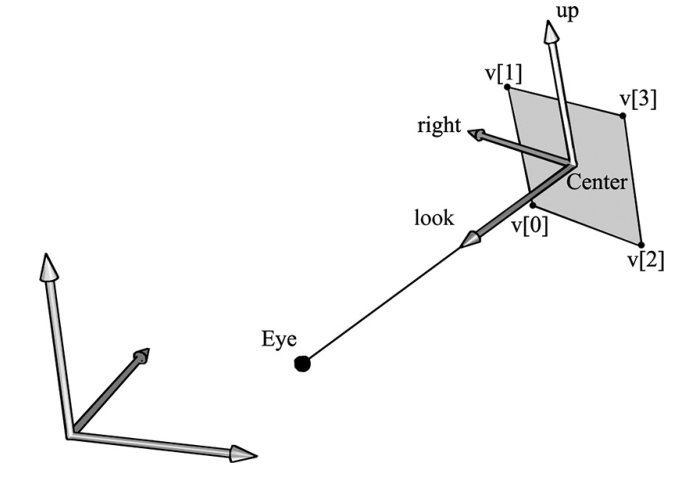
\includegraphics[width=\textwidth]{12-4}
    \centering
    \caption{从本地坐标系统和广告牌的世界大小计算广告牌四边形顶点。}
    \label{fig:12-4}
\end{figure}

\begin{figure}[h]
    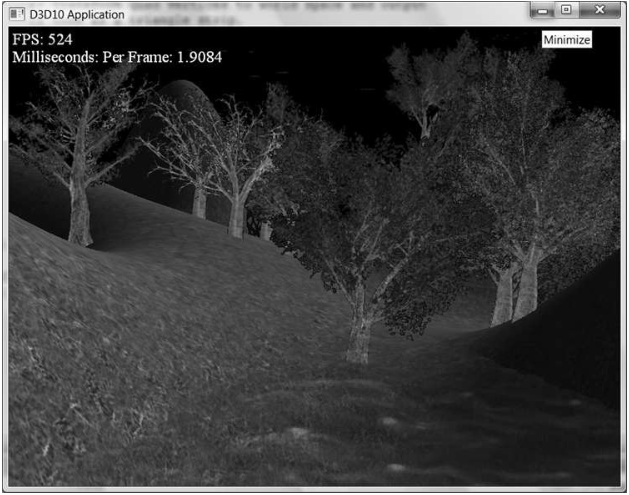
\includegraphics[width=\textwidth]{12-5}
    \centering
    \caption{树广告牌演示截图}
    \label{fig:12-5}
\end{figure}

\begin{flushleft}
请注意,广告牌的局部坐标系对于每个广告牌都不同,因此必须为每个广告牌计算。\\

对于本演示,我们将构建一个点基元列表(PSO的PrimitiveTopologyType的D3D12\_PRIMITIVE\_TOPOLOGY\_TYPE\_POINT和作为ID3D12GraphicsCommandList::IASetPrimitiveTopology的参数的D3D\_PRIMITIVE\_TOPOLOGY\_POINTLIST)略高于陆地平面(land mass)。 这些点代表我们想要绘制的广告牌的中心。 在几何着色器中,我们将这些点扩展为广告牌四边形。 此外,我们将在几何着色器中计算广告牌的世界矩阵。 图\ref{fig:12-5}显示了演示的屏幕截图。\\

如图\ref{fig:12-5}所示,此示例构建了第10章的“Blend”演示。\\

~\\
NOTICE: 广告牌的常见CPU实现是在动态顶点缓冲区(即上载堆)中每个广告牌使用四个顶点。 然后每次相机移动时,顶点都会在CPU上更新并存储到GPU缓冲区,以便广告牌面向相机。 此方法必须将每个广告牌的四个顶点提交到IA阶段,并且需要更新具有开销的动态顶点缓冲区。 使用几何着色器方法,可以利用静态顶点缓冲区,几何着色器执行广告牌扩展并使广告牌面向相机。 此外,广告牌的内存占用量非常小,只需要将每个广告牌的一个顶点提交到IA阶段即可。
~\\
\end{flushleft}

%-------- 12.2.2 --------
\subsection{顶点结构(Vertex Structure)}
\begin{lstlisting}
struct TreeSpriteVertex
{
    XMFLOAT3 Pos;
    XMFLOAT2 Size;
};

mTreeSpriteInputLayout =
{
    {"POSITION", 0, DXGI_FORMAT_R32G32B32_FLOAT, 0, 0,
                 D3D12_INPUT_CLASSIFICATION_PER_VERTEX_DATA, 0},
    {"SIZE",     0, DXGI_FORMAT_R32G32_FLOAT, 0, 12,
                 D3D12_INPUT_CLASSIFICATION_PER_VERTEX_DATA, 0}
};
\end{lstlisting}

\begin{flushleft}
顶点(vertex)存储一个点(point),该点表示广告牌在世界空间中的中心位置。它还包括一个尺寸分量,它存储广告牌的宽度/高度(按比例缩放到世界空间单位);也就是几何着色器知道扩展后广告牌应该有多大(图\ref{fig:12-6})。通过使每个顶点的尺寸不同,我们可以轻松地容纳不同尺寸的广告牌。\\
\end{flushleft}

\begin{figure}[h]
    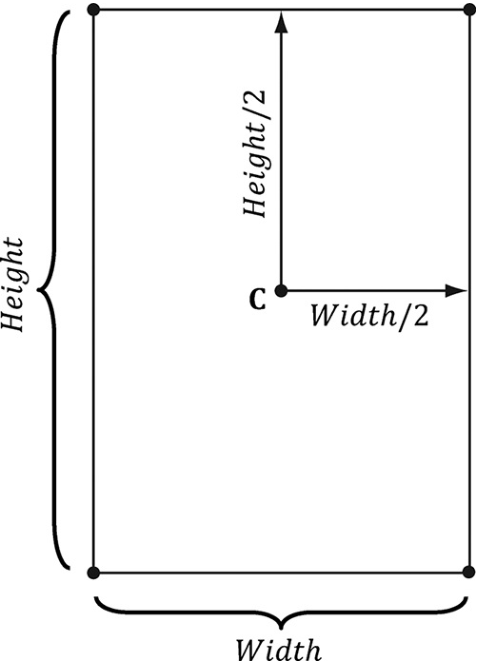
\includegraphics[width=\textwidth]{12-6}
    \centering
    \caption{将一个点扩展为四边形。}
    \label{fig:12-6}
\end{figure}

\begin{flushleft}
除了纹理数组(第12.2.4节)之外,"Tree Billboard"演示中的其他C++代码现在应该是常规的Direct3D代码(创建顶点缓冲区,效果,调用绘制方法等)。因此,我们现在将注意力转向TreeSprite.hlsl文件。
\end{flushleft}

%-------- 12.2.3 --------
\subsection{对应的HLSL文件(The HLSL File)}
\begin{flushleft}
由于这是我们的第一个带有几何着色器的演示,我们将在此处显示整个HLSL文件,以便您可以看到它如何与顶点和像素着色器组合在一起。这个效果还引入了一些我们尚未讨论过的新对象(SV_PrimitiveID和Texture2DArray);这些项目将在下面讨论。目前,主要关注几何着色器程序GS;此着色器将一个点扩展为与面向摄像机的世界y轴对齐的四边形,如12.2.1中所述。\\
\end{flushleft}

\begin{lstlisting}
//************************************************************
// TreeSprite.hlsl by Frank Luna (C) 2015 All Rights Reserved.
//************************************************************

// Defaults for number of lights.
#ifndef NUM_DIR_LIGHTS
    #define NUM_DIR_LIGHTS 3
#endif

#ifndef NUM_POINT_LIGHTS
    #define NUM_POINT_LIGHTS 0
#endif

#ifndef NUM_SPOT_LIGHTS
    #define NUM_SPOT_LIGHTS 0
#endif

// Include structures and functions for lighting.
#include "LightingUtil.hlsl"

Texture2DArray gTreeMapArray : register(t0);


SamplerState gsamPointWrap        : register(s0);
SamplerState gsamPointClamp       : register(s1);
SamplerState gsamLinearWrap       : register(s2);
SamplerState gsamLinearClamp      : register(s3);
SamplerState gsamAnisotropicWrap  : register(s4);
SamplerState gsamAnisotropicClamp : register(s5);

// Constant data that varies per frame.
cbuffer cbPerObject : register(b0)
{
    float4x4 gWorld;
    float4x4 gTexTransform;
};

// Constant data that varies per material.
cbuffer cbPass : register(b1)
{
    float4x4 gView;
    float4x4 gInvView;
    float4x4 gProj;
    float4x4 gInvProj;
    float4x4 gViewProj;
    float4x4 gInvViewProj;
    float3 gEyePosW;
    float cbPerObjectPad1;
    float2 gRenderTargetSize;
    float2 gInvRenderTargetSize;
    float gNearZ;
    float gFarZ;
    float gTotalTime;
    float gDeltaTime;
    float4 gAmbientLight;

    float4 gFogColor;
    float gFogStart;
    float gFogRange;
    float2 cbPerObjectPad2;

    // Indices [0, NUM_DIR_LIGHTS) are directional lights;
    // indices [NUM_DIR_LIGHTS, NUM_DIR_LIGHTS+NUM_POINT_LIGHTS) are point lights;
    // indices [NUM_DIR_LIGHTS+NUM_POINT_LIGHTS, NUM_DIR_LIGHTS+NUM_POINT_LIGHT+NUM_SPOT_LIGHTS)
    // are spot lights for a maximum of MaxLights per object.
    Light gLights[MaxLights];
};

cbuffer cbMaterial : register(b2)
{
    float4   gDiffuseAlbedo;
    float3   gFresnelR0;
    float    gRoughness;
    float4x4 gMatTransform;
};
 
struct VertexIn
{
    float3 PosW  : POSITION;
    float2 SizeW : SIZE;
};

struct VertexOut
{
    float3 CenterW : POSITION;
    float2 SizeW   : SIZE;
};

struct GeoOut
{
    float4 PosH    : SV_POSITION;
    float3 PosW    : POSITION;
    float3 NormalW : NORMAL;
    float2 TexC    : TEXCOORD;
    uint   PrimID  : SV_PrimitiveID;
};

VertexOut VS(VertexIn vin)
{
    VertexOut vout;

    // Just pass data over to geometry shader.
    vout.CenterW = vin.PosW;
    vout.SizeW   = vin.SizeW;

    return vout;
}
 
 // We expand each point into a quad (4 vertices), so the maximum number of vertices
 // we output per geometry shader invocation is 4.
[maxvertexcount(4)]
void GS(point VertexOut gin[1], 
        uint primID : SV_PrimitiveID, 
        inout TriangleStream<GeoOut> triStream)
{   
    //
    // Compute the local coordinate system of the sprite relative to the world
    // space such that the billboard is aligned with the y-axis and faces the eye.
    //

    float3 up = float3(0.0f, 1.0f, 0.0f);
    float3 look = gEyePosW - gin[0].CenterW;
    look.y = 0.0f; // y-axis aligned, so project to xz-plane
    look = normalize(look);
    float3 right = cross(up, look);

    //
    // Compute triangle strip vertices (quad) in world space.
    //
    float halfWidth  = 0.5f*gin[0].SizeW.x;
    float halfHeight = 0.5f*gin[0].SizeW.y;
    
    float4 v[4];
    v[0] = float4(gin[0].CenterW + halfWidth*right - halfHeight*up, 1.0f);
    v[1] = float4(gin[0].CenterW + halfWidth*right + halfHeight*up, 1.0f);
    v[2] = float4(gin[0].CenterW - halfWidth*right - halfHeight*up, 1.0f);
    v[3] = float4(gin[0].CenterW - halfWidth*right + halfHeight*up, 1.0f);

    //
    // Transform quad vertices to world space and output 
    // them as a triangle strip.
    //
    
    float2 texC[4] = 
    {
        float2(0.0f, 1.0f),
        float2(0.0f, 0.0f),
        float2(1.0f, 1.0f),
        float2(1.0f, 0.0f)
    };
    
    GeoOut gout;
    [unroll]
    for(int i = 0; i < 4; ++i)
    {
        gout.PosH     = mul(v[i], gViewProj);
        gout.PosW     = v[i].xyz;
        gout.NormalW  = look;
        gout.TexC     = texC[i];
        gout.PrimID   = primID;
        
        triStream.Append(gout);
    }
}

float4 PS(GeoOut pin) : SV_Target
{
    float3 uvw = float3(pin.TexC, pin.PrimID%3);
    float4 diffuseAlbedo = gTreeMapArray.Sample(gsamAnisotropicWrap, uvw) * gDiffuseAlbedo;

#ifdef ALPHA_TEST
    // Discard pixel if texture alpha < 0.1.  We do this test as soon 
    // as possible in the shader so that we can potentially exit the
    // shader early, thereby skipping the rest of the shader code.
    clip(diffuseAlbedo.a - 0.1f);
#endif

    // Interpolating normal can unnormalize it, so renormalize it.
    pin.NormalW = normalize(pin.NormalW);

    // Vector from point being lit to eye. 
    float3 toEyeW = gEyePosW - pin.PosW;
    float distToEye = length(toEyeW);
    toEyeW /= distToEye; // normalize

    // Light terms.
    float4 ambient = gAmbientLight*diffuseAlbedo;

    const float shininess = 1.0f - gRoughness;
    Material mat = { diffuseAlbedo, gFresnelR0, shininess };
    float3 shadowFactor = 1.0f;
    float4 directLight = ComputeLighting(gLights, mat, pin.PosW,
        pin.NormalW, toEyeW, shadowFactor);

    float4 litColor = ambient + directLight;

#ifdef FOG
    float fogAmount = saturate((distToEye - gFogStart) / gFogRange);
    litColor = lerp(litColor, gFogColor, fogAmount);
#endif

    // Common convention to take alpha from diffuse albedo.
    litColor.a = diffuseAlbedo.a;

    return litColor;
}
\end{lstlisting}

%-------- 12.2.4 --------
\subsection{SV_PrimitiveID}
\begin{flushleft}
此示例中的几何着色器采用带有语义 SV_PrimitiveID 的特殊无符号整数参数。
\end{flushleft}

\begin{lstlisting}[escapechar=^]
[maxvertexcount(4)]
void GS(point VertexOut gin[1],
    ^\textbf{uint primID : SV_PrimitiveID,}^
    inout TriangleStream<GeoOut> triStream)
\end{lstlisting}

\begin{flushleft}
指定此语义时,它会告诉输入汇编程序阶段为每个基元自动生成基元 ID。当执行绘制调用以绘制$n$个基元时,第一个基元标记为$0$;第二个基元标记为$1$;依此类推,直到绘制调用中的最后一个原语标记为$n-1$。原始ID仅对于单个绘制调用是唯一的。在我们的广告牌示例中,几何着色器不使用此ID(尽管几何着色器可以);相反,几何着色器将基元ID写入传出顶点,从而将其传递到像素着色器阶段。像素着色器使用基元ID索引到纹理数组,这在下一章节说明。\\

~\\
NOTICE: 如果不存在几何着色器,则可以将原始ID参数添加到像素着色器的参数列表中:\\
\end{flushleft}

\begin{lstlisting}
float4 PS(VertexOut pin, 
    uint primID : SV_PrimitiveID) : SV_Target
{
    // Pixel shader body...
}
\end{lstlisting}

\begin{flushleft}
但是,如果存在几何着色器,则基元ID参数必须出现在几何着色器签名中。然后,几何着色器可以使用基元ID或将其传递给像素着色器阶段(或两者)。\\

输入汇编程序也可以生成顶点ID。为此,请使用语义SV\_VertexID 向顶点着色器签名添加类型为 uint 的参数:\\
\end{flushleft}

\begin{lstlisting}
VertexOut VS(VertexIn vin, uint vertID : SV_VertexID)
{
    // vertex shader body...
}
\end{lstlisting}

\begin{flushleft}
对于Draw调用,draw 调用中的顶点将使用$0,1,...,n-1$中的ID进行标记,其中$n$是绘制调用中的顶点数。对于DrawIndexed调用,顶点ID对应于顶点索引值。\\
\end{flushleft}

%-------- 12.3 --------
\section{纹理数组(Texture Arrays)}
%-------- 12.3.1 -------
\subsection{概览(Overview)}
\begin{flushleft}
纹理数组存储纹理数组。 在C++代码中,纹理数组由 ID3D12Resource 接口表示,就像所有资源(纹理和缓冲区)一样。 在创建 ID3D12Resource 对象时,实际上有一个名为 DepthOrArraySize 的属性可以设置为指定纹理需要存储的纹理元素的数量(或3D纹理的深度)。 当我们在d3dApp.cpp中创建深度/模板纹理时,我们总是将其设置为1.如果查看Common/DDSTextureLoader.cpp 中的 CreateD3DResources12 函数,您将看到代码如何支持创建纹理数组和体积纹理。 在HLSL文件中,纹理数组由 Texture2DArray 类型表示:\\
\end{flushleft}

\begin{lstlisting}
Texture2DArray gTreeMapArray;
\end{lstlisting}

\begin{flushleft}
现在,你可能会疑惑为什么我们需要纹理数组的数据结构。为什么不直接这样做:\\
\end{flushleft}

\begin{lstlisting}
Texture2D TexArray[4];
...
float4 PS(GeoOut pin) : SV_Target
{
    float4 c = TexArray[pin.PrimID%4].Sample(samLinear, pin.Tex);
\end{lstlisting}

\begin{flushleft}
在着色器模型5.1(Direct3D 12的新功能)中,我们实际上可以做到这一点。 但是,以前的Direct3D版本不允许这样做。 此外,这样的索引纹理可能会有一些开销,具体取决于硬件,因此在本章中我们将坚持使用纹理数组数据结构。\\
\end{flushleft}

%-------- 12.3.2 -------
\subsection{采样纹理数组(Sampling a Texture Array)}
\begin{flushleft}
在Billboards演示中,我们使用以下代码对纹理数组进行采样:\\
\end{flushleft}

\begin{lstlisting}
float3 uvw = float3(pin.Tex, pin.PrimID%4);
float4 diffuseAlbedo = gTreeMapArray.Sample(
    gsamAnisotropicWrap, uvw) * gDiffuseAlbedo;
\end{lstlisting}

\begin{flushleft}
使用纹理数组时,需要三个纹理坐标。 前两个纹理坐标是通常的2D纹理坐标; 第三个纹理坐标是纹理数组的索引。 例如,0是数组中第一个纹理的索引,1是数组中第二个纹理的索引,2是数组中第三个纹理的索引,依此类推。\\
在Billboards演示中,使用带有四个纹理元素的纹理数组,每个纹理元素都有不同的树纹理(图\ref{fig:12-7})。 但是,因为我们每次绘制调用绘制的树数超过四棵,所以原始ID将大于三。 因此,采用原始ID与4取模(pin.PrimID%4)将原始ID映射到0,1,2或3,它们是具有四个元素的数组的有效数组索引。\\
\end{flushleft}

\begin{figure}[h]
    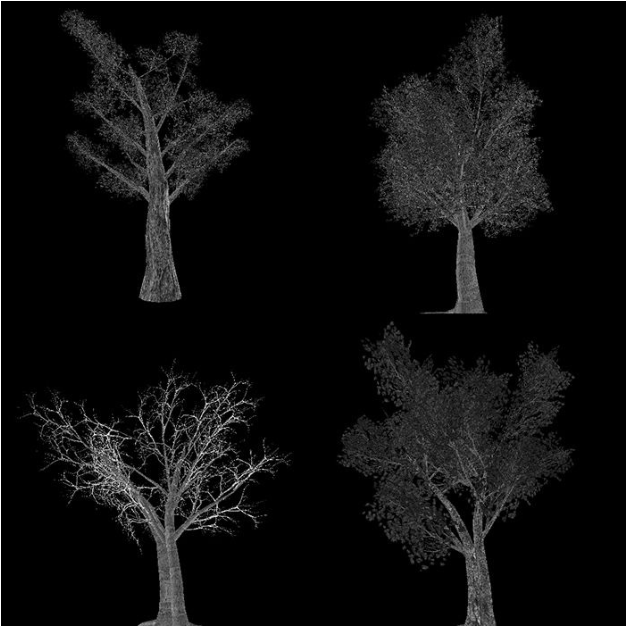
\includegraphics[width=\textwidth]{12-7}
    \centering
    \caption{树广告牌图像}
    \label{fig:12-7}
\end{figure}

\begin{flushleft}
纹理数组的一个优点是我们能够在一次绘制调用中绘制具有不同纹理的基元集合。 通常,我们必须为每个具有不同纹理的网格物体设置单独的渲染项:\\
\end{flushleft}

\begin{lstlisting}
SetTextureA();
DrawPrimitivesWithTextureA();
SetTextureB();
DrawPrimitivesWithTextureB();
...
SetTextureZ();
DrawPrimitivesWithTextureZ();
\end{lstlisting}

\begin{flushleft}
每个set和draw调用都有一些与之相关的开销。 使用纹理数组,我们可以将其减少为一组和一个绘制调用:\\
\end{flushleft}

\begin{lstlisting}
SetTextureArray();
DrawPrimitivesWithTextureArray();
\end{lstlisting}

%-------- 12.3.3 -------
\subsection{加载纹理数组(Loading Texture Array)}
\begin{flushleft}
在Common/DDSTextureLoader.h/.cpp 中的DDS加载代码支持加载存储纹理数组的DDS文件。 所以关键是要创建一个包含纹理数组的DDS文件。 为此,我们使用Microsoft提供的texassemble工具,网址为 https://directxtex.codeplex.com/wikipage?title=Texassemble&referringTitle=Texconv。 以下语法展示如何从4个图像t0.dds,t1.dds,t2.dds和t3.dds创建名为treeArray.dds的纹理数组:\\
\end{flushleft}

\begin{lstlisting}
texassemble -array -o treeArray.dds t0.dds t1.dds t2.dds t2.dds
\end{lstlisting}

\begin{flushleft}
请注意,使用texassemble构建纹理数组时,输入图像应该只有一个mipmap级别。 在调用texassemble构建纹理数组之后,可以使用texconv(https://directxtex.codeplex.com/wikipage?title=Texconv)生成mipmap并根据需要更改像素格式:\\
\end{flushleft}

\begin{lstlisting}
texconv -m 10 -f BC3_UNORM treeArray.dds
\end{lstlisting}

%-------- 12.3.4 -------
\subsection{纹理子资源(Texture Subresources)}
\begin{flushleft}
现在我们已经讨论了纹理数组,接下来可以讨论子资源了。 图\ref{fig:12-8}显示了具有多个纹理的纹理数组的示例。 反过来,每个纹理都有自己的mipmap链。 Direct3D API使用术语数组切片来引用纹理中的元素及其完整的mipmap链。 Direct3D API使用术语mip slice来指代纹理数组中特定级别的所有mipmap。子资源是指纹理数组元素中的单个mipmap级别。\\
\end{flushleft}

\begin{figure}[h]
    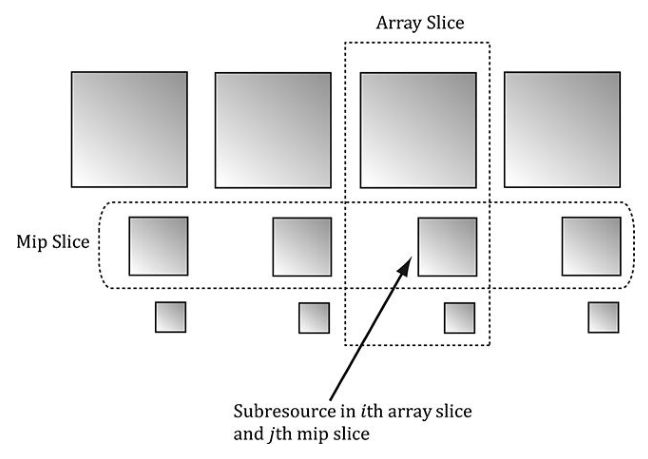
\includegraphics[width=\textwidth]{12-8}
    \centering
    \caption{带有四个纹理的纹理数组。 每个纹理都有三个mipmap级别。}
    \label{fig:12-8}
\end{figure}

\begin{flushleft}
给定纹理数组索引和mipmap级别,我们可以访问纹理数组中的子资源。 子资源也可以用线性索引标记; Direct3D使用一个有序的线性索引,如图\ref{fig:12-9}所示。\\
\end{flushleft}

\begin{figure}[h]
    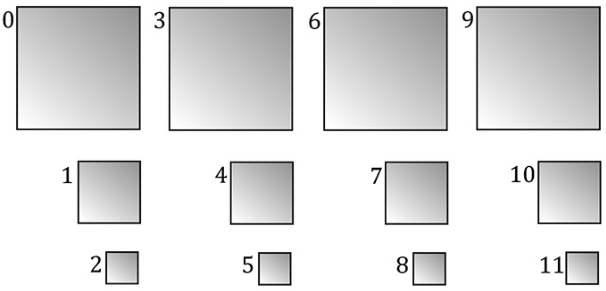
\includegraphics[width=\textwidth]{12-9}
    \centering
    \caption{用线性索引标记的纹理数组中的子资源。}
    \label{fig:12-9}
\end{figure}

\begin{flushleft}
以下工具方法用于计算mip级别,数组索引和mipmap级别数量的线性子资源索引:\\
\end{flushleft}

\begin{lstlisting}
inline UINT D3D12CalcSubresource(
    UINT MipSlice, 
    UINT ArraySlice,
    UINT PlaneSlice, 
    UINT MipLevels, 
    UINT ArraySize)
{
    return MipSlice + ArraySlice * MipLevels + 
           PlaneSlice * MipLevels * ArraySize;
}
\end{lstlisting}

%-------- 12.4 -------
\section{Alpha-to-Coverage}
\begin{flushleft}
当运行“树广告牌”演示时,请注意在某些距离处,树广告牌剪裁的边缘看起来是块状的。 这是由剪辑功能引起的,我们用它来掩盖不属于树的纹理像素; 剪辑功能要么保留一个像素,要么拒绝它——没有平滑的过渡。 从眼睛到广告牌的距离会因为短距离导致放大,这使得块变得更大,并且短距离导致使用更低分辨率的mipmap级别。\\

解决此问题的一种方法是使用透明度混合而不是alpha测试。 由于线性纹理过滤,边缘像素将略微模糊,从白色(不透明像素)到黑色(屏蔽像素)平滑过渡。因此,透明度混合将导致沿着边缘从不透明像素到遮罩像素的平滑淡出。 不幸的是,透明度混合需要按照从前到后的顺序进行排序和渲染。 排序少量树状广告牌的开销并不高,但如果我们渲染森林或草原草地,排序操作可能很昂贵,因为必须在每一帧完成; 更糟糕的是,按照从前到后的顺序渲染会导致大量透支(参见第11章中的练习8),这可能会造成性能下降。\\

有人可能会建议 MSAA(多重采样抗锯齿——参见4.1.7)提供帮助,因为 MSAA 用于平滑多边形的块状边缘。 确实,它应该有些用处 ,但存在问题。MSAA 在像素中心每像素执行一次像素着色器,然后根据可见性(每个子像素评估深度/模板测试)和覆盖范围(子像素中心位于多边形内部或外部)(与其子像素共享该颜色信息?)。这里的关键是覆盖是在多边形级别确定的。 因此,MSAA不会检测由alpha通道定义的树状广告牌切口的边缘——它只会查看纹理映射到的四边形的边缘。 那么有没有办法告诉Direct3D在计算覆盖范围时考虑alpha通道? 答案是肯定的,我们采用称为alpha-to-coverage的技术即可。\\

启用 MSAA 并启用 alpha-to-coverage(D3D12\_BLEND\_DESC::AlphaToCoverageEnable=true 的成员)时,硬件将查看像素着色器返回的alpha值,并使用它来确定coverage [NVIDIA05]。 例如,对于4X MSAA,如果像素着色器alpha为0.5,那么我们可以假设四个子像素中的两个被覆盖,这将会创建平滑的边缘。\\

一般的建议是,你总是希望使用 alpha-to-coverage 来覆盖 alpha 遮罩的剪切纹理,如树叶和栅栏。 它需要启用 MSAA。 请注意,在我们的演示应用程序的构造函数中,设置:\\
\end{flushleft}

\begin{lstlisting}
mEnable4xMsaa = true;
\end{lstlisting}

\begin{flushleft}
这使我们的示例框架创建了支持4X MSAA的 back 和 depth 缓冲区。
\end{flushleft}

%-------- 12.5 -------
\section{总结}
\begin{flushleft}
1.假设我们没有使用曲面细分阶段,几何着色器阶段是位于顶点和像素着色器阶段之间的可选阶段。 为通过输入汇编器发送的每个基元调用几何着色器。 几何着色器可以输出零个,一个或多个基元。 输出基元类型可以与输入基元类型不同。 在离开几何着色器之前,应将输出基元的顶点转换为齐次空间。 从几何着色器输出的基元接下来进入渲染管道的光栅化阶段。 几何着色器编入了效果文件中,并排顶点和像素着色器。\\

2.广告牌技术是使用具有物体图像的四边形纹理而不是物体的真实3D模型。对于远处的物体,观察者无法分辨出正在使用的广告牌。 广告牌的优势在于,当纹理四边形足够时,GPU不必浪费渲染完整3D对象的处理时间。 此技术可用于渲染树木的森林,其中真正的3D几何图形用于相机附近的树木,广告牌用于远处的树木。为了使广告牌技术起作用,广告牌必须始终面向相机。广告牌技术可以在几何着色器中有效实现。\\

3.可以将类型为 uint 和语义 SV\_PrimitiveID 的特殊参数添加到几何着色器的参数列表中,如以下示例所示:\\
\end{flushleft}

\begin{lstlisting}
[maxvertexcount(4)]
void GS(point VertexOut gin[1],
    uint primID : SV_PrimitiveID,
    inout TriangleStream<GeoOut> triStream);
\end{lstlisting}

\begin{flushleft}
指定此语义时,它会告诉输入汇编程序阶段为每个基元自动生成基元ID。 当执行绘制调用以绘制n个基元时,第一个基元标记为$0$; 第二个原语标记为$1$; 依此类推,直到绘制调用中的最后一个原语标记为$n-1$。 如果不存在几何着色器,则可以将原始ID参数添加到像素着色器的参数列表中。 但是,如果存在几何着色器,则基本ID参数必须出现在几何着色器签名中。 然后,几何着色器可以使用基元ID或将其传递给像素着色器阶段(或两者)。\\

4.输入汇编程序阶段可以生成顶点ID。 为此,请使用语义 SV\_VertexID 向顶点着色器签名添加类型为uint的参数。 对于Draw调用,draw调用中的顶点将使用 $0,1,...,n-1$ 中的ID进行标记,其中$n$是绘制调用中的顶点数。对于 DrawIndexed 调用,顶点ID对应于顶点索引值。\\

5.纹理数组结构存储纹理数组数据。在 C++ 代码中,纹理数组由 ID3D12Resource 接口表示,就像所有资源(纹理和缓冲区)一样。在创建 ID3D12Resource 对象时,有一个名为 DepthOrArraySize 的属性,可以将其设置为指定纹理存储的纹理元素的数量(或3D纹理的深度)。在HLSL中,纹理数组由 Texture2DArray 类型表示。使用纹理数组时,需要三个纹理坐标。前两个纹理坐标是通常的2D纹理坐标;第三个纹理坐标是纹理数组的索引。例如,$0$是数组中第一个纹理的索引,$1$是数组中第二个纹理的索引,$2$是数组中第三个纹理的索引,依此类推。纹理数组的一个优点是我们能够在一次绘制调用中绘制具有不同纹理的基元集合。每个基元将具有纹理数组的索引,该索引指示要应用于基元的纹理。\\

6.Alpha-to-coverage指示硬件在确定子像素覆盖时查看像素着色器返回的alpha值。 这样可以实现alpha遮罩剪裁纹理(如树叶和栅栏)的平滑边缘。 Alpha到覆盖范围由PSO中的 D3D12\_BLEND\_DESC::AlphaToCoverageEnable 字段控制。\\
\end{flushleft}


%-------- 12.6 -------
\section{练习}
\begin{flushleft}
1.考虑在$xz$平面中用线条绘制的圆。使用几何着色器将线条扩展为无盖的圆柱体。\\
2.二十面体是球体的粗略近似。通过细分每个三角形(图\ref{fig:12-10}),并将新顶点投影到球体上,可以获得更好的近似效果。(将顶点投影到单位球体上只需要对位置向量进行标准化,因为所有单位向量的头部都与单位球体的表面重合。)对于本练习,构建并渲染二十面体。使用几何着色器根据距离相机的距离$d$细分二十面体。例如,如果$d<15$,则将原始二十面体细分两次;如果$15\leq d < 30$,则将原二十面体细分一次;如果$d\geq 30$,那么只需渲染原始的二十面体。如果物体靠近相机,只使用大量的多边形;如果物体很远,那么较粗糙的网格就足够了,我们不需要浪费GPU功率来处理比需要更多的多边形。图\ref{fig:12-10}显示了线框和实线(点亮)模式中并排显示的三个LOD级别。有关对二十面体进行曲面细分的讨论,请参阅7.4.3。\\
\end{flushleft}

\begin{figure}[h]
    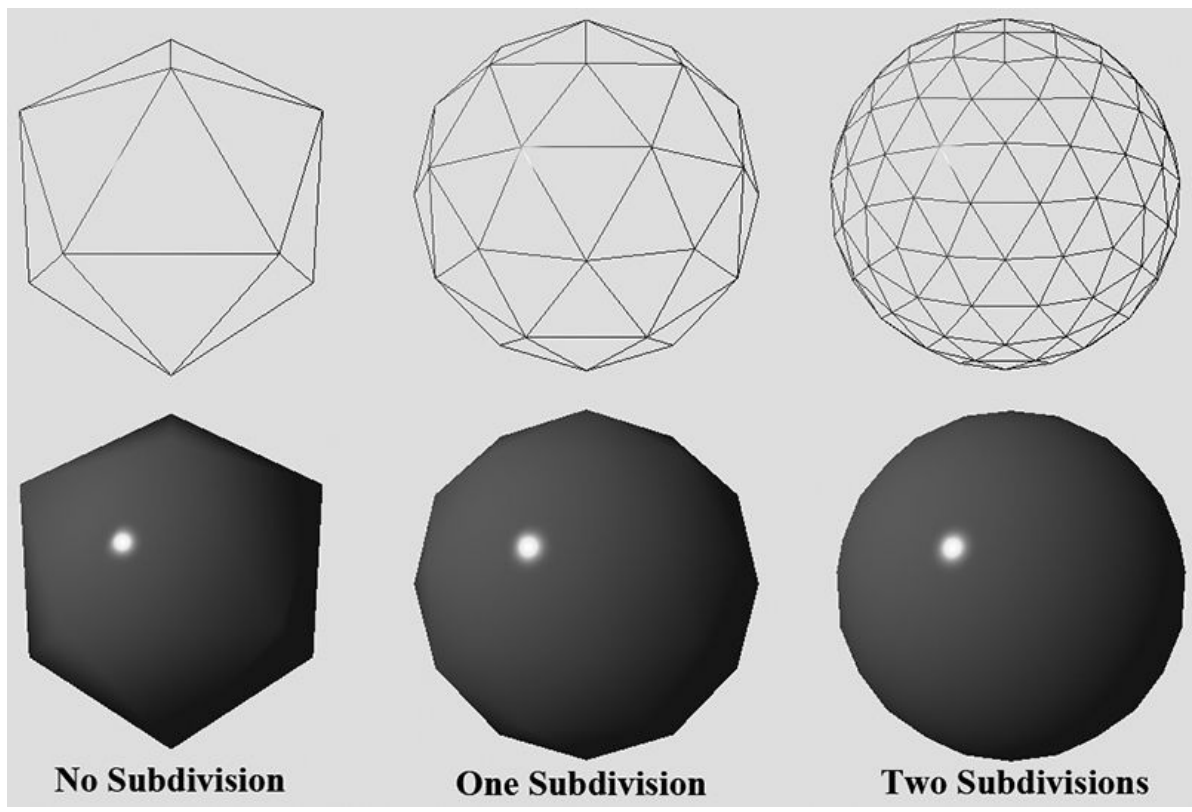
\includegraphics[width=\textwidth]{12-10}
    \centering
    \caption{将顶点投影到单位球面上的二十面体细分过程。}
    \label{fig:12-10}
\end{figure}

\begin{flushleft}
3.简单的爆炸效果可以通过面部法线方向上的三角形相对于时间进行平移的函数来模拟。此模拟可以在几何着色器中实现。 对于输入到几何着色器中的每个三角形,几何着色器计算面法线$n$,然后根据爆炸开始后的时间$t$在$n$方向上平移三个三角形顶点$p_{0}$,$p_{1}$和$p_{2}$:\\
\edn{flushleft}

\begin{lstlisting}
p_{i}^{'}=p_{i}+tn,i=0,1,2
\end{lstlisting}

\begin{flushleft}
面法线$n$可以不是单位长度,并且可以相应地缩放以控制爆炸的速度。人们甚至可以使缩放取决于原始ID,以便每个基元以不同的速度传播。使用二十面体(未细分)作为样本网格来实现此效果。\\

4.本练习很有用,可用于调试可视化网格的顶点法线。编写一种效果,将网格的顶点法线渲染为短线段。为此,请实现几何着色器,该几何着色器输入网格的点基元(即,其顶点拓扑类型为D3D\_PRIMITIVE\_TOPOLOGY\_POINTLIST),以便每个顶点都通过几何着色器进行泵送(pumped through)。 现在,几何着色器可以将每个点扩展为某个长度为$L$的线段。如果顶点具有位置$p$和法线$n$,则表示顶点法线的线段的两个端点是$p$和$p+Ln$。 实现此操作后,正常绘制网格,然后使用法线矢量可视化技术再次绘制场景,以便在场景顶部渲染法线。 使用“Blend”演示作为测试场景。\\

5.与上一个练习类似,编写一个效果,将网格的面法线渲染为短线段。对于此效果,几何着色器将输入三角形,计算其法线,并输出线段。\\

6.此练习显示,对于Draw调用,绘制调用中的顶点将使用$0,1,...,n-1$中的ID进行标记,其中$n$是绘制调用中的顶点数,以及DrawIndexed调用的顶点数,顶点ID对应于顶点索引值。 按以下方式修改“Tree Billboards”演示。 首先,将顶点着色器更改为以下内容:\\
\end{flushleft}

\begin{lstlisting}
VertexOut VS(
    VertexIn vin, 
    uint vertID : SV_VertexID)
{
    VertexOut vout;
    // Just pass data over to geometry shader.
    vout.CenterW = vin.PosW;
    vout.SizeW = float2(2+vertID, 2+vertID);
    return vout;
}
\end{lstlisting}

\begin{flushleft}
换句话说,我们根据其中心的顶点ID来调整树广告牌的大小。现在运行该程序; 当绘制$16$个广告牌时,大小应该在$2$到$17$之间。现在修改图形如下:不是使用单个绘制调用一次绘制所有$16$个点,而是使用四个:\\
\end{flushleft}

\begin{lstlisting}
cmdList->Draw(4, 0, 0, 0);
cmdList->Draw(4, 0, 4, 0);
cmdList->Draw(4, 0, 8, 0);
cmdList->Draw(4, 0, 12, 0);
\end{lstlisting}

\begin{flushleft}
现在运行程序。这次,大小应该在$2$到$5$之间。因为每个绘制调用绘制$4$个顶点,所以每个绘制调用的顶点ID范围为$0-3$。 现在使用索引缓冲区和四个DrawIndexed调用。 运行程序后,大小应返回到$2$到$17$的范围。这是因为使用DrawIndexed时,顶点ID对应于顶点索引值。\\

7.按以下方式修改“Tree Billboards”演示。首先,从像素着色器中删除“modulo 4”:\\
\end{flushleft}

\begin{lstlisting}
float3 uvw = float3(pin.Tex, pin.PrimID);
\end{lstlisting}

\begin{flushleft}
现在运行程序。由于我们绘制了$16$个基元,原始ID范围为$0-15$,因此这些ID超出了数组边界。但是,这不会导致错误,因为越界索引将被限制为最高有效索引(在这种情况下为3)。现在不是使用单个绘制调用一次绘制所有$16$个点,而是像这样使用四个:\\
\end{flushleft}

\begin{lstlisting}
cmdList->Draw(4, 0, 0, 0);
cmdList->Draw(4, 0, 4, 0);
cmdList->Draw(4, 0, 8, 0);
cmdList->Draw(4, 0, 12, 0);
\end{lstlisting}

\begin{flushleft}
再次运行该程序。这次没有夹紧。因为每个绘制调用绘制$4$个基元,所以每个绘制调用的原始ID范围为$0-3$。 因此,原始ID可以用作索引而不会越界。这表明每次绘制调用时原始ID“count”重置为零。\\
\end{flushleft}